\subsection{Direct five-entry Burgers learning and distributed readout}
\label{sec:direct_burgers_protocol}

This experiment replaces the prescribed three-coefficient Burgers learner in
its role as main-paper evidence. The earlier coefficient-family experiment
remains a separate historical protocol. Here every entry of a local differential
row is learned directly from observed context-rate incompatibility; the physical
Burgers coefficient family is used only to generate and evaluate the plant.
The protocol was fixed before running the five initializations and subsequent
sensor and timestep conditions. The main figure uses the preselected seed 732
and spatial site 0, without selection by the outcome.

\subsubsection{Plant, observations, and free differential row}
On the periodic domain $s\in[0,2\pi)$, the simulator is
\begin{equation}
 w_t+w w_s-.08w_{ss}-u=0,
 \qquad z=(w,w_s,w_{ss},u,w_t).
 \label{eq:direct_burgers_plant}
\end{equation}
A 32-point Fourier collocation grid and RK4 advance the physical state with
piecewise-linear $u$. All spatial points are sensed and actuated. The initial
state is $w(s,0)=.2+.015\sin s$, with $u(s,0)=0$. Fixed identity context scales
are used. At each site the learner stores an independent row
$q\in\mathbb R^{1\times5}$ and a $5\times5$ memory matrix. Every entry of $q$
is initialized from a generic Gaussian draw, followed by unit normalization.
The five initial seeds are 732--736; the independent sensor seed is the initial
seed plus 100000. No coefficient estimate, known partial entry, sparse physical
pattern, physical eigenspace, or true-$F$ initialization is supplied.

In the ideal condition, $w$ and $w_t$ are measured exactly; spatial channels
are spectral derivatives of the measured field. This is an explicit ideal
sensor assumption, not a noisy position-only result. The learner does not
receive an exact $w_{tt}$ sensor: its observation is the causal context secant
\begin{equation}
 v_k=\frac{z(t_k)-z(t_k-.05)}{.05},\qquad t_{k+1}-t_k=.005\,\mathrm{s}.
 \label{eq:direct_burgers_observation}
\end{equation}
After the first valid history window, it integrates
\begin{equation}
 \begin{aligned}
 \dot R&=v_kv_k^T-R/4,\\
 \dot q&=-10^4\{qR-(qRq^T)q\},\qquad qq^T=1.
 \end{aligned}
 \label{eq:direct_burgers_law}
\end{equation}
The secant is held during the current $.005$-s observation interval, but the
memory evolves throughout the representation update. Each RK4 stage evaluates
\begin{equation}
 R(t_k+\delta)=e^{-\delta/4}R_k+
               4(1-e^{-\delta/4})v_kv_k^T.
 \label{eq:direct_burgers_memory}
\end{equation}
At least four subdivisions are used; their length $d$ obeys
$10^4d\max\{\operatorname{tr}R_k,\operatorname{tr}R_{k+1}\}\leq.25$
across sites. Unit normalization follows each subdivision. This is numerical
integration of the coupled law, not replacement of learning by a bottom
eigenvector or descent with a frozen memory matrix.

\subsubsection{Training and same-field rate completion}
For $0\leq t<80$ s the input-rate probe is
\begin{equation}
 \begin{aligned}
 \dot u&=.01\sum_{k=0}^{3}\omega_k
       \sin((k+1)s+.37k)\cos(\omega_kt),\\
 &(\omega_0,\ldots,\omega_3)=(3,5,7,11).
 \end{aligned}
 \label{eq:direct_burgers_probe}
\end{equation}
Before observing $t=80$ s, the complete plant, input, learned row, memory,
observation histories and random-number state are cloned. One arm continues
learning and the other holds $q$ fixed. Both act on their own physical
trajectories until $t=100$ s. The fixed arm may evolve a diagnostic memory;
that memory does not update its row.

The target is
\begin{equation}
 w_d=.2+.015\sin s\cos(.3t)+.01\cos(2s)\sin(.5t).
 \label{eq:direct_burgers_reference}
\end{equation}
At each controlled sample, measured channels and the pre-update row form the
query before the current secant is assimilated. Set
\begin{equation}
 a_d=(w_d)_{tt}-4(w-w_d)-4(w_t-(w_d)_t).
\end{equation}
The supplied rates are $v_S=(w_t,(w_t)_s,(w_t)_{ss},a_d)$ and the computed
channel is $v_C=\dot u$. The same learned row returns
\begin{equation}
 \dot u=-\frac{q_w w_t+q_{w_s}(w_t)_s+q_{w_{ss}}(w_t)_{ss}+q_{w_t}a_d}{q_u}.
 \label{eq:direct_burgers_completion}
\end{equation}
A query with $|q_u|<.1$ uses the declared model-independent input decay $-u$
and is counted as guarded, not successful learned completion. Applied input
rates are clipped to $[-5,5]$; $\max_s|w|>5$ stops a branch. There is no
physical-model fallback. The ideal cohort has no guarded or clipped controlled
sample and no stopped branch; its smallest controlled $|q_u|$ is $.67137$.

\subsubsection{Separate recovery, compatibility, and task scores}
Only the evaluator forms the physical row
$F=(w_s,w,-.08,-1,1)$ at each branch's actual clean context. Let
$p=F/\|F\|$. The physical recovery metric is
\begin{equation}
 e_F=\|q^Tq-p^Tp\|_F=\sqrt{2(1-(qp^T)^2)}.
 \label{eq:direct_burgers_score}
\end{equation}
It is invariant to row sign and scale and ranges from zero to $\sqrt2$.
Entry plots use unit normalization and evaluator-only sign alignment; this
display convention never changes the learner or controller. Pre-update
incompatibility is scored separately as $\frac12(qv_k)^2$. Task RMS is the
root mean square of $w-w_d$ over all sites and applied observations in the
specified window. Terminal commands at $t=100$ are stored but not applied and
are excluded from task/readout metrics. Rendering uses every fifth sample;
metrics use every applied sample without smoothing.

\begin{figure}[t]
 \centering
 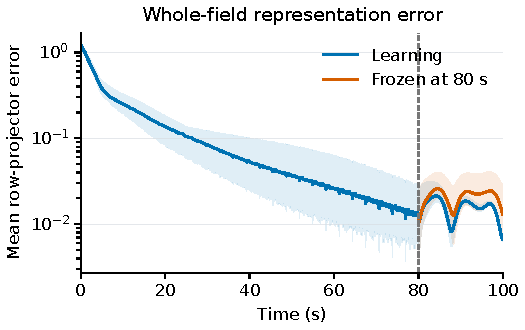
\includegraphics[width=\columnwidth]{figures/direct_burgers_diagnostics.pdf}
 \caption{Whole-field Burgers representation error, complementing the main
figure's partial, incompatibility and control plots. Curves are means and bands
span all five seeds, with error averaged over all 32 spatial sites. At 80 s,
the shared probing trajectory branches into separately controlled adaptive
and frozen runs. The adaptive rows continue learning through 100 s;
the frozen rows retain their values at 80 s.}
\label{fig:direct_burgers_protocol}
\end{figure}

\begin{table*}[t]
\centering
\caption{All ideal main-cohort outcomes. Late means/RMS use $[96,100)$ s.
The training qualification uses $[76,80)$ s and all the criteria stated in the text.
The final row gives the across-seed mean $\pm$ sample standard deviation.}
\label{tab:direct_burgers_ideal}
\renewcommand{\arraystretch}{1.15}
\begin{tabular}{c c c c c c}
\hline
Seed & Training qualified & Adaptive $e_F$ & Frozen $e_F$ &
Adaptive task RMS ($10^{-6}$) & Frozen task RMS ($10^{-6}$)\\
\hline
732 & No & .013761 & .018433 & 8.5084 & 22.4895\\
733 & No & .013222 & .021239 & 8.5186 & 25.8758\\
734 & Yes & .013231 & .014272 & 8.4460 & 11.7942\\
735 & No & .014729 & .037314 & 8.9005 & 49.9873\\
736 & Yes & .013344 & .015503 & 8.4874 & 13.9083\\
\hline
All five & 2/5 & $.013658\pm.000638$ & $.021352\pm.009323$ &
$8.5722\pm.1856$ & $24.8110\pm15.2371$\\
\hline
\end{tabular}
\end{table*}

The prospective training qualification requires mean $e_F\leq.05$, pooled
95th percentile $\leq.1$, maximum $\leq.25$, worst-site mean $\leq.1$, and
mean error at most one quarter of the initial-row same-stream error. Only
seeds 734 and 736 pass every condition. All five pass the inherited weaker
mean/reduction check and all five pass the declared adaptive late conditions:
mean $e_F\leq.1$, 95th percentile $\leq.25$, task RMS $\leq10^{-3}$,
guard and clipping fractions each strictly below $.01$, and completion to
100 s. These are offline labels, never training stops or feedback gates.
The five-seed result therefore demonstrates continued direct learning and
readout, not uniformly qualified tracking after convergence.

Over the full $[80,100)$ control interval, adaptive and frozen task RMS are
$.001223645\pm.000000231$ and $.001223943\pm.000000617$, respectively.
Their common initial transition dominates this interval; the late advantage
must not be described as a large full-horizon improvement. For the two
qualified seeds, frozen readout already works well and continued learning
provides a modest late improvement. The remaining seeds include continuing
recovery from incomplete training.

Even ideal sensing does not make the finite secant exactly tangent to the
instantaneous physical relation. The physical unit-row half-mean-square
secant energy is $4.4414\times10^{-11}$ over $[76,80)$ and averages
$1.5610\times10^{-13}$ on the adaptive late trajectories. The latter learned
energy is $3.6992\times10^{-10}$. Thus neither numerical zero compatibility
nor exact physical identification is claimed. The local time-varying rows
need not define an integrable global Jacobian field.

\subsubsection{Sensor failures and numerical refinement}
The complete study retains 19 cases: five ideal, five causal-clean and five
causal-noisy main cases, plus two ideal and two causal-clean refinements.
In causal cases a quadratic endpoint least-squares fit to the preceding $.10$
s of measured positions estimates $w_t$; the same estimate supplies both the
context and controller. No future samples or true-rate fill are used. Noisy
cases add independent position noise with standard deviation $10^{-5}$ per
site/sample. The causal secant first becomes valid at $.15$ s. Noise and row
initializations vary together across the five paired seeds; this is not a
crossed factorial noise study.

\begin{table}[t]
\centering
\caption{Main-cohort outcomes, retaining every seed. ``Late pass'' requires
all combined adaptive recovery, task, guard and completion criteria.}
\label{tab:direct_burgers_conditions}
\renewcommand{\arraystretch}{1.15}
\begin{tabular}{lccc}
\hline
Sensing & Training qualified & Late pass & Complete A/F\\
\hline
Ideal & 2/5 & 5/5 & 5/5, 5/5\\
Causal clean & 0/5 & 0/5 & 5/5, 0/5\\
Causal noisy & 0/5 & 0/5 & 5/5, 5/5\\
\hline
\end{tabular}
\end{table}

Every causal-clean frozen main branch reaches the declared field bound at
83.2 s. The two causal-clean frozen refinements stop at 83.2 and 83.2025 s.
Failed observations and unexecuted commands remain in the raw records; absent
late windows are not extrapolated. The causal-clean training discrepancy is
principally a biased observed covariance target: for seed 732 the learned,
observed-bottom and clean-bottom physical errors are $.479532$, $.480820$
and $.004098$, respectively. Small observed incompatibility does not identify
the physical partials. In the noisy cohort, adaptive late mean physical error
is $1.41362$, task RMS is $.007956$, and the guard fraction is one. Continued
adaptation under that sensor model is not successful partial recovery.

For preselected seed 732, the whole-loop step is halved from $.005$ to $.0025$
and $.00125$ s, keeping physical windows fixed. Ideal late mean field changes
are $2.11605\times10^{-5}$ and $9.60095\times10^{-6}$; the first exceeds the
prospective absolute $10^{-5}$ sensitivity flag, while neither exceeds the
10\% relative flag. Worst-site training means $.104301$, $.100618$ and
$.098807$ cross the qualification boundary only at the finest step. That
favorable result does not replace the prespecified main-cohort count of 2/5.
The second causal-clean halving changes late field error by 18.70\% and task
RMS by 38.39\%, so its whole-loop sensitivity test fails. Halving the loop
changes sensing, sampling and control as well as integration; it is not a
pure solver-order or continuous-PDE convergence test.

\subsubsection{Reproduction and audit boundary}
The portable package is
\path{experiments/direct_submission/burgers/}.
Its \path{protocol.json} preserves the original prospective declaration;
\path{source_mapping.json} distinguishes unchanged scientific functions from
local import, command-line and provenance adaptations. The package includes
compact full-sample plot trajectories, selected complete original chunks and
checkpoints, and all-condition summaries. These selected files are not the
complete 6.63-GB original raw archive, which remains a separate artifact;
no public download location is implied here.

The independent final-pass reconstruction checks the hashes of all 610 ideal
raw chunks and reproduces 200 metric comparisons. Every controlled command
is reconstructed from the saved pre-update row and observed supplied rates;
the largest discrepancy is $1.39\times10^{-17}$. Portable-source replay of
600 archived samples across training, adaptive and frozen phases is bitwise
identical. An independent literal joint-$q/R$ ODE check gives a row discrepancy
$1.51\times10^{-10}$, with successive held-observation halving errors
$9.29\times10^{-12}$ and $5.77\times10^{-13}$. The historical independent
audit also retains all 19 cases, sensor/filter reconstruction, coupled-ODE
checks and failed branch records.

From the package directory, \path{verify_package.py} performs the focused
replay/numerical checks, \path{plot_figure_focus.py} regenerates the current
figures without simulation, \path{burgers_direct.py} reproduces one declared case or the complete
study in a new directory, and \path{audit_runs.py} independently reconstructs
raw runs without importing the learner or simulator. The README gives exact
commands and dependencies. These numerical checks verify implementation and
provenance; they do not establish global identifiability, sensor robustness,
off-trajectory integrability or closed-loop stability.
